% One nondimensional equation, three geometries, one shape index s.
% Fourth of four composite figures for Lecture 7 (collocation), authored
% 2026-09-08.
%
% WHAT IT SHOWS, and where it comes from.  Sec. "Transient conduction" of
% ../../optimization-private/lecture-notes/lectures/collocation.tex rescales
% rho Cp dT/dt = div(k grad T) with T' = (T-T0)/(Tinf-T0), r' = r/R and
% t' = alpha t / R^2 -- "every physical parameter drops out" -- and lands on
% Eq. (7-geomfamily):
%
%     dT/dt = d2T/dr2 + (s/r) dT/dr,    s = 0 slab, 1 cylinder, 2 sphere
%
% with T(0,r) = 0, T(t,1) = 1, dT/dr(t,0) = 0.  Source: Kantor, ND Pyomo
% Cookbook, 05.03-Heat_Conduction_in_Various_Geometries.ipynb.
%
% The figure's job is to make "one equation, three geometries" visible: the
% three cross-sections differ only in how many directions heat can leave, and
% s counts exactly that.  Hence the "s = number of curved directions" gloss
% under the panels -- slab conducts in one direction, cylinder in two, sphere
% in three, and s = (dimensions) - 1.
%
% 🔴 r = 0 IS THE CENTRE, NOT AN EDGE, in all three panels.  The lecture's
% activity turns on this: the equation is singular at r = 0 for s > 0 while the
% solution is not, because symmetry gives dT/dr = 0 there and s/r dT/dr is 0/0.
% The symmetry line/axis/centre is therefore marked identically in all three
% drawings, and labelled with the boundary condition rather than with "r = 0"
% alone.  Do not redraw the slab as a half-slab with r = 0 on its left face --
% that would make it the odd one out and lose the shared reading.
%
% GREYSCALE.  The three geometries are told apart by SHAPE, which no printer
% can flatten.  Colour is used only twice and redundantly: the surface (r = 1)
% carries a VERY THICK rule and an orange tint, the symmetry line/axis/centre
% carries a DASH-DOT rule and a blue tint.  Okabe-Ito blue #0072B2 (L* = 46)
% and orange #E69F00 (L* = 70.6), dL* = 24.6.  Nothing is carried by colour
% alone.
%
% TIKZ LIBRARIES.  Base tikz plus >=stealth.  No calc, no patterns, no
% decorations.pathreplacing -- the sphere's equator and the cylinder's end caps
% are plain \draw ellipse and \draw arc.  Builds under both preambles.

\definecolor{cpblue}{HTML}{0072B2}
\definecolor{cporange}{HTML}{E69F00}

\begin{tikzpicture}[x=1cm, y=1cm, font=\small,
  surf/.style   = {cporange, line width=2.2pt},
  sym/.style    = {cpblue, thick, dash pattern=on 6pt off 2pt on 1pt off 2pt},
  rarrow/.style = {->, >=stealth, thick},
]

% =====================================================================
% PANEL 1 -- SLAB, s = 0.  A rectangle; heat leaves through two parallel
% faces.  r is measured from the mid-plane to either face.
% =====================================================================
\node[align=center, font=\small] at (1.6,3.55) {\textbf{Slab}\\ $s = 0$};

\draw[thick, fill=black!5] (0.4,0.5) rectangle (2.8,2.9);
\draw[surf] (0.4,0.5) -- (0.4,2.9);
\draw[surf] (2.8,0.5) -- (2.8,2.9);
\draw[sym]  (1.6,0.28) -- (1.6,3.12);

\draw[rarrow] (1.6,1.7) -- (2.8,1.7);
\node[above, font=\scriptsize, inner sep=2pt] at (2.2,1.72) {$r$};
\fill[cpblue] (1.6,1.7) circle (2.2pt);
\node[cporange, right, font=\scriptsize, inner sep=3pt] at (2.82,2.55) {$T=1$};

% =====================================================================
% PANEL 2 -- CYLINDER, s = 1.  Drawn in three dimensions (two end ellipses
% and two generators) so it cannot be mistaken for the sphere in print.
% Heat leaves radially, in two directions.
% =====================================================================
\node[align=center, font=\small] at (6.4,3.55) {\textbf{Cylinder}\\ $s = 1$};

% Curved wall, then the visible top rim.
\draw[surf] (5.2,2.6) -- (5.2,0.9);
\draw[surf] (7.6,2.6) -- (7.6,0.9);
\draw[thick, fill=black!5] (6.4,2.6) ellipse (1.2 and 0.42);
\draw[surf] (5.2,0.9) arc (180:360:1.2 and 0.42);
\draw[thick, densely dotted] (5.2,0.9) arc (180:0:1.2 and 0.42);

\draw[sym] (6.4,3.15) -- (6.4,0.35);
\draw[rarrow] (6.4,2.6) -- (7.6,2.6);
\node[above, font=\scriptsize, inner sep=2pt] at (7.05,2.6) {$r$};
\fill[cpblue] (6.4,2.6) circle (2.2pt);
\node[cporange, right, font=\scriptsize, inner sep=3pt] at (7.62,1.75) {$T=1$};

% =====================================================================
% PANEL 3 -- SPHERE, s = 2.  Circle plus an equator ellipse, which is what
% separates it from the cylinder at a glance.  Heat leaves in three
% directions.
% =====================================================================
\node[align=center, font=\small] at (11.2,3.55) {\textbf{Sphere}\\ $s = 2$};

\draw[thick, fill=black!5] (11.2,1.7) circle (1.2);
\draw[surf] (11.2,1.7) circle (1.2);
\draw[thick, densely dotted] (11.2,1.7) ellipse (1.2 and 0.4);
\fill[cpblue] (11.2,1.7) circle (2.6pt);
\draw[sym] (11.2,1.7) -- (10.0,1.7);

\draw[rarrow] (11.2,1.7) -- (12.09,2.51);
\node[above left, font=\scriptsize, inner sep=1pt] at (11.85,2.2) {$r$};
\node[cporange, right, font=\scriptsize, inner sep=3pt] at (12.42,2.6) {$T=1$};

% =====================================================================
% SHARED CAPTION -- the one equation, and the conditions that are the same in
% all three panels.  Kept in ONE place rather than repeated per panel: that
% repetition is exactly what the shape index removes.
% =====================================================================
\draw[black!35] (0.2,-0.45) -- (12.6,-0.45);

\node[align=center] at (6.4,-1.05)
  {$\dfrac{\partial T}{\partial t}
     = \dfrac{\partial^2 T}{\partial r^2}
     + \dfrac{s}{r}\,\dfrac{\partial T}{\partial r}$};

\node[align=center, font=\scriptsize] at (6.4,-2.25)
  {\textcolor{cpblue}{\textbf{-- $\cdot$ --} \ $r = 0$: symmetry,
      $\partial T / \partial r = 0$}
   \qquad
   \textcolor{cporange}{\rule[0.35ex]{9pt}{1.6pt} \ $r = 1$: surface, $T = 1$}
   \qquad
   $t = 0$: $T = 0$};

\node[align=center, font=\scriptsize\itshape] at (6.4,-2.85)
  {one equation, one parameter --- $s$ counts the curved directions};

\end{tikzpicture}
